\subsection{Hardware}

Unabhängig von der Zusammenstellung umfänglicher Speicherlösungen, müssen die Daten trotzdem irgendwann auf einen Hardwarespeicher geschrieben werden. Folgender Abschnitt erläutert, die allgemeine Funktion und geht auf einige der am häufigsten verwendeten Typen ein.

\todo{Beschreibe die Funktion von Blockstorage, Unterscheidung RAM / Harddisk}

\begin{figure}[hbt]
	\centering
	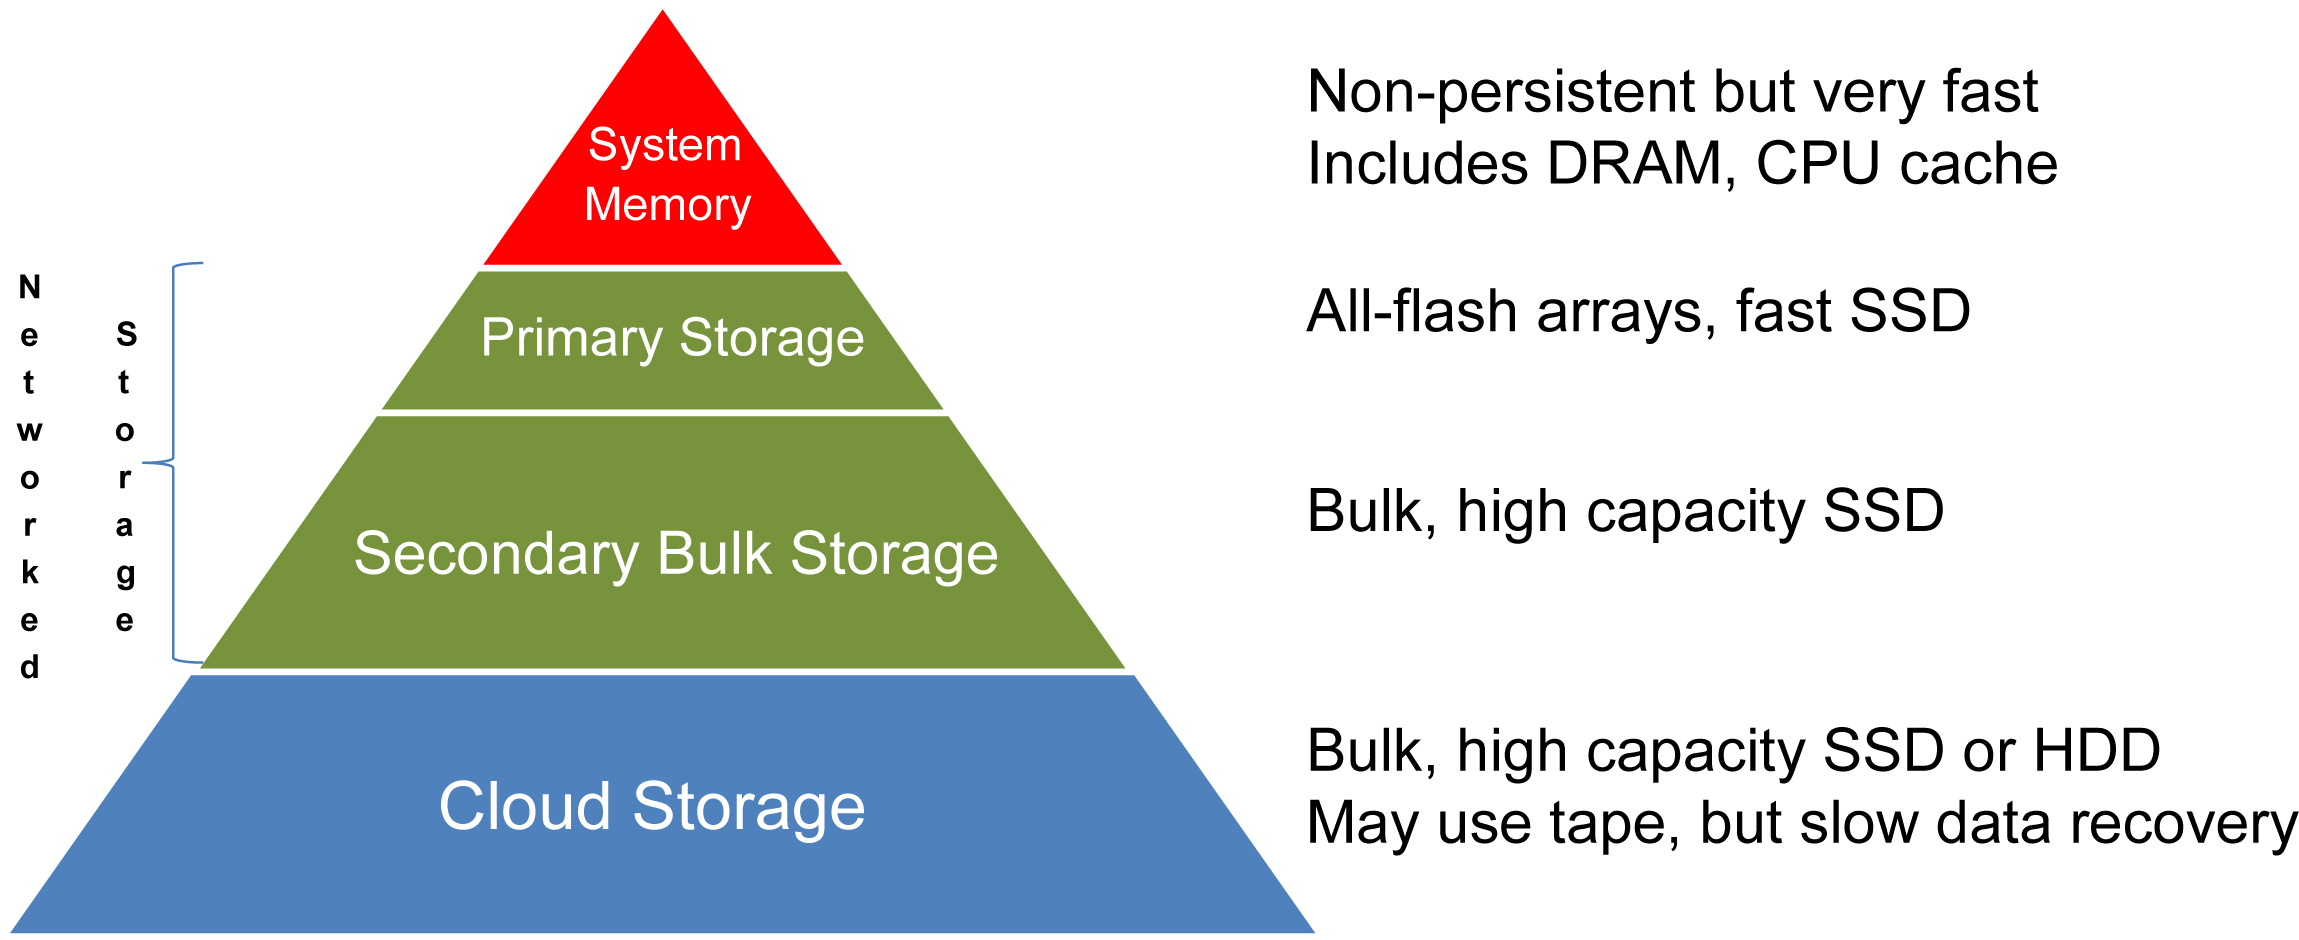
\includegraphics[scale=0.75]{images/storage-pyramide}
	\caption{Speicher Pyramide \parencite{kaufmann.2016}}
	\label{fig:storagepyramide}
\end{figure}

\subsubsection{Hard Disk Drive (HDD)}

Hierbei handelt es sich um einen nicht volatilen Speicher, der digital kodierten Inhalte auf der magnetischen Oberfläche einer Platte speichert. Traditionell gibt es zwei Protokolle: SAS im kommerziellen Sektor und SATA im privaten \parencite{wikibooks.2016}.

Ein oder mehrere Leseköpfe werden mithilfe von Armen und einem Servomotor über die Platte bewegt, um relevante Stellen auszulesen. Bei der Herstellung von HDDs werden Tracks in die Platte geschrieben, die jeweils ein Label und Blockinformationen besitzen. Durch sie ist es einfacher den Lesekopf zu platzieren. Jeder dieser Tracks kann bis zu einigen MBs an Daten beinhalten. Durch die Blockbildung bei I/O Operationen kann häufig nur ein einzelner Block (64-256) Block geschrieben werden, wodurch Festplatten unnötig langsam werden. Durch neue Technologie können IOs gequeued, sodass die Platte kontinuierlich lesen und schreiben kann. Trotzdem ist nur eine maximale Geschwindigkeit von ungefähr 300 \gls{IOPS} das Limit für Platten mit 10.000 RPM.  \parencite{kaufmann.2016}.

Jede Festplatte hat heutzutage einige private Sektoren, auf denen Reparatur Informationen und Reserveblöcke gespeichert sind. Fällt ein Block in der Festplatte aus (durch zum Beispiel physikalische Beschädigung), kann dieser fließend ersetzt werden, sodass keine Daten verloren gehen. Kurz vor dem Ausfall einer Platte steigt diese Anzahl der Lesefehler einer Platte massiv an, sodass eine Datenreovery versucht werden kann. Leider ist dies keine verlässliche Methode, um Daten zu sichern, sodass andere Methoden verwendet werden sollten \parencite{kaufmann.2016}.

Um Datenverlust durch Plattenausfälle entgegenzuwirken, besteht die Möglichkeit der Verwendung von so genannten RAIDs. Dies ist eine Methode, bei der mehrere HDDs so zusammengeschaltet werden, sodass bei dem Ausfall einer Einzelner die Daten weiterhin verfügbar sind \parencite{wikibooks.2016}.

Festplatten sind gut erforscht, es treten extrem selten unbekannte Probleme auf und werden seit Jahrzehnten verwendet, ihr Speicher ist extrem günstig geworden und in Masse verfügbar. Ihr größter Nachteil ist eine sehr geringe I/O Geschwindigkeit im Vergleich mit neueren Technologien \parencite{kaufmann.2016}.

\subsubsection{Solid State Drive (SSD)}

In 2007 wurde der erste SSD Speicher vermarktet und stach durch extrem hohe Zugriffszahlen heraus. Diese sind waren bei 4000 \gls{IOPS} bereits um das zehnfache höher als die klassischer Festplatten. Heutzutage ist es möglich IOPS Zahlen im Millionenbereich zu erreichen, was eine Revolution für Speicher bedeutet \parencite{kaufmann.2016}.

\begin{figure}[hbt]
	\centering
	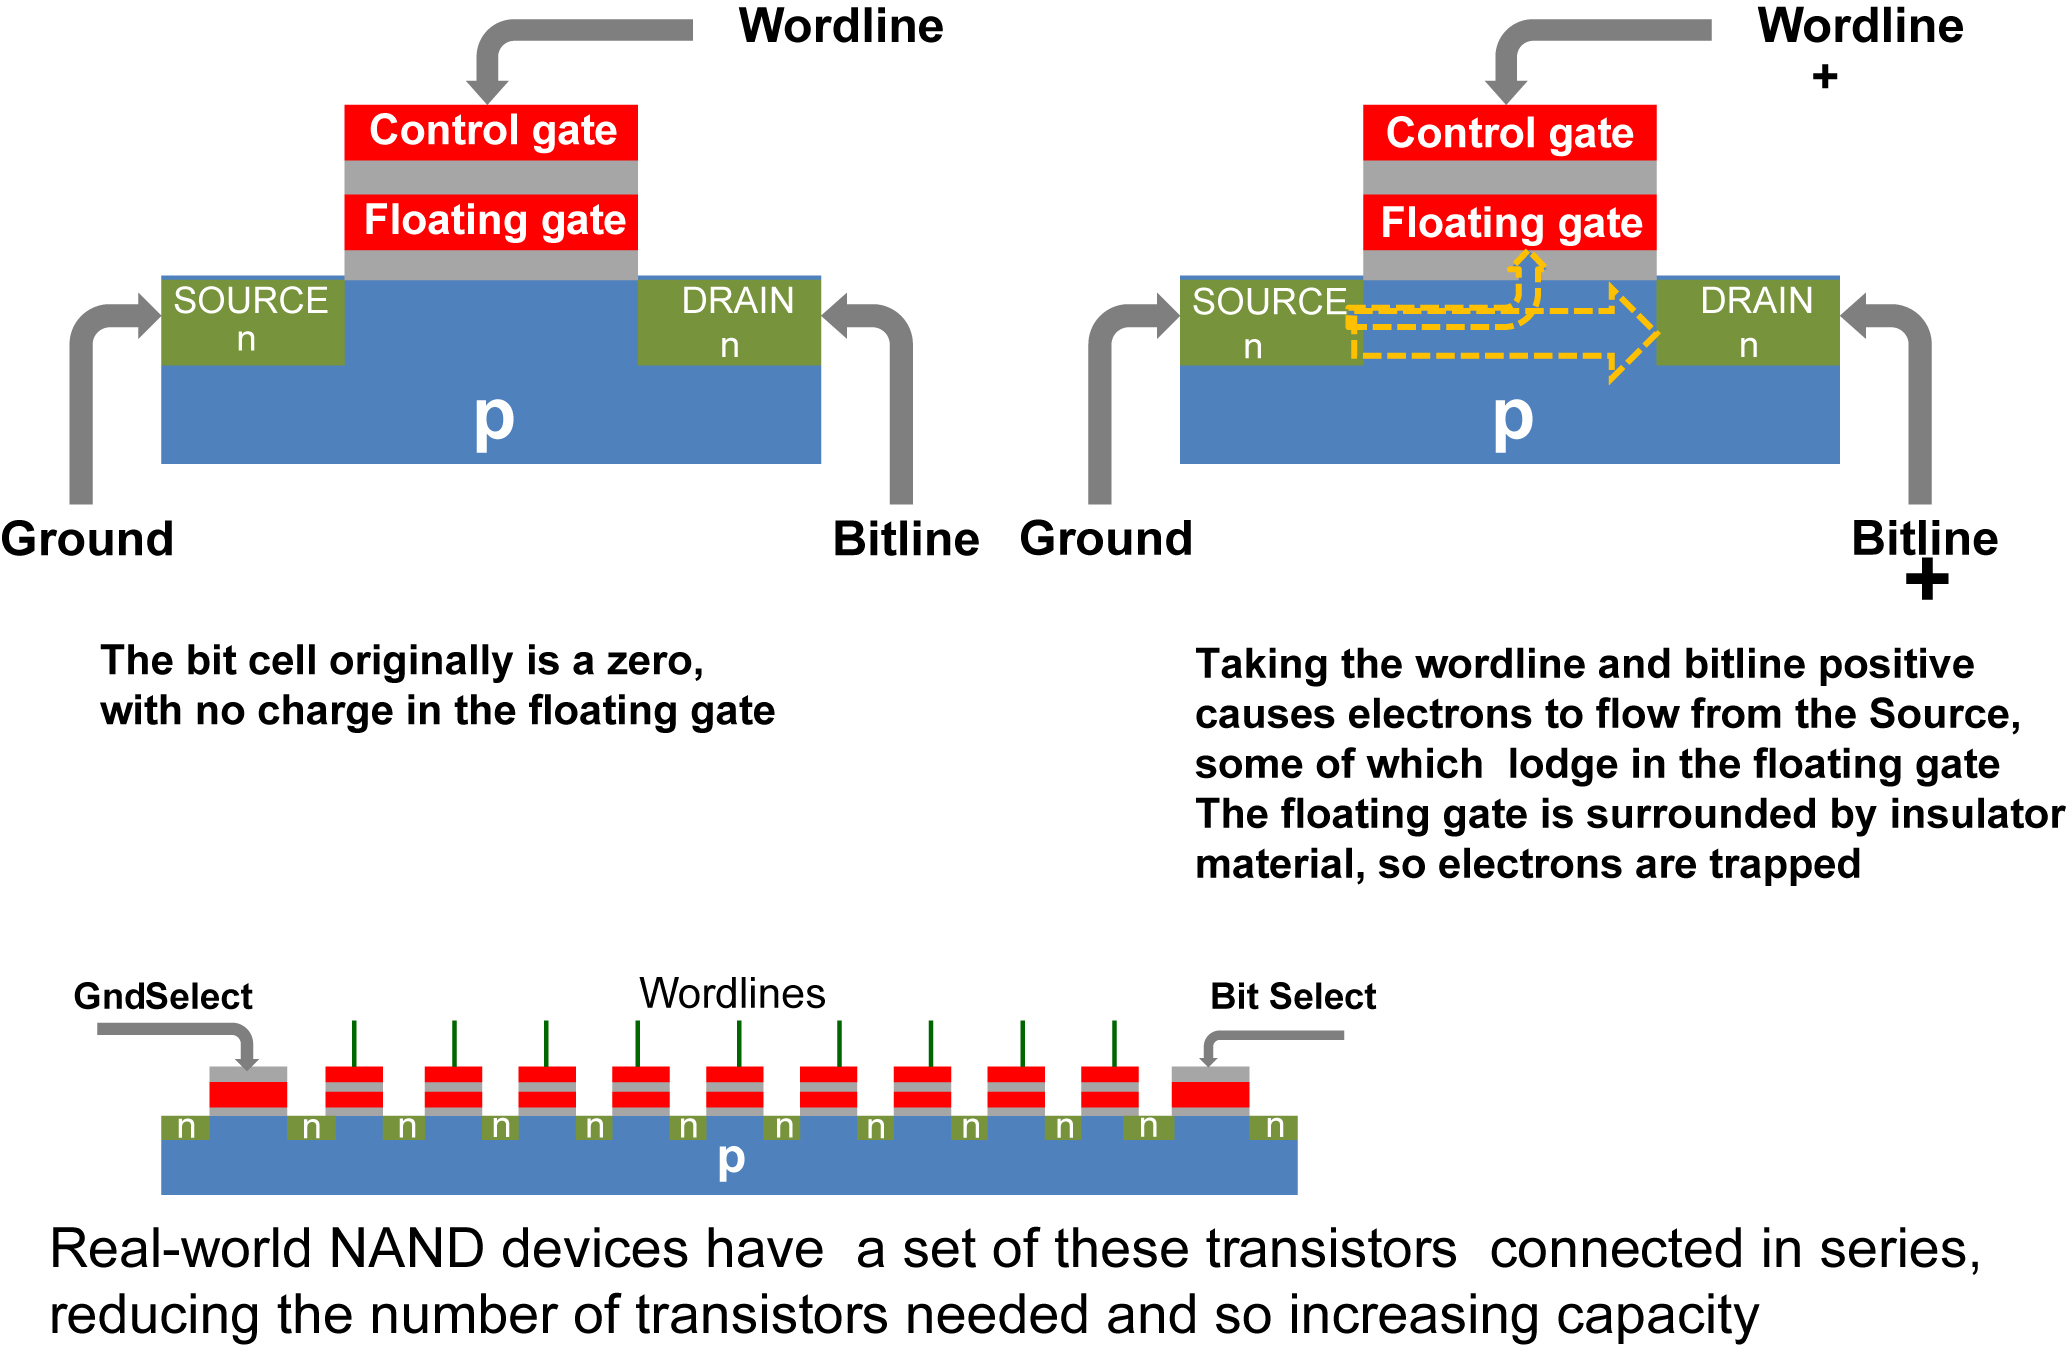
\includegraphics[scale=0.85]{images/flash}
	\caption{Funktionsweise eines NAND Flash Speichers \parencite{kaufmann.2016}}
	\label{fig:flash}
\end{figure}

SSDs benutzen Nicht-Und (NAND) memory chips zum Speichern einzelner Bitinformationen. Von diesen Zellen gibt es dann einige Millionen, die beliebig adressiert werden können (Random Access Memory). Innerhalb eines so genannten Floating Gate können nun Elektronen eingefangen werden, um eine binäre Eins zu repräsentieren. Im Ausgangszustand sind diese ``Fallen'' leer, um einen Nullinformationen zu speichern. Sobald der Speichercontroller eine Zellen laden will, wird der Einlasstransistor geöffnet und einige Elektronen in der Zelle für eine beliebig lange Zeit gefangen.

Dieser Prozess findet in \autoref{fig:flash} statt, wenn auf der Bit- und Wordline eine positive Ladung gesetzt wird. Meistens liegen mehrere Zellen auf einer Reihe, was den Lese Prozess verkomplizieren kann. Es wird eine niedrige Spannung an alle Wordlines angelegt, wodurch bei geladenen Zellen eine Konduktivität festgestellt werden kann. 

Wird eine einzelne Zelle zu häufig beschrieben, kann diese Isolation verlieren, wodurch sie unnutzbar zum Speichern wird. Schreibstrategien und Reservezellen werden verwendet, um dies vorzubeugen.	

Zum Löschen der Zellen wird eine hohe negativer Spannung an die Zellen angelegt, wodurch die gefangenen Elektronen aus den Floating Gates heraus gedrückt werden. Dies passiert meistens in fest definierten Pages, sodass keine speziellen Blöcke gelöscht werden können. Nach dem Löschen eines Blockes wird dessen Zeiger auf eine vorher geleerte Page bewegt und der Block als ``discared'' markiert. Sind innerhalb einer Page genug Blöcke in diesem Zustand, werden die verbleibenden Daten verschoben und die gesamte Page gelöscht und Teil des freien Speichers der SSD \parencite{kaufmann.2016}. 
Durch diesen Prozess ist das Löschen von Dateien nicht mehr zuverlässig, da die Daten noch für lange Zeit innerhalb eines ``discared'' Blockes liegen können, der erst wesentlich später, vom Controller gelöscht wird.

SSDs können über das SATA Protokoll angeschlossen werden, aber in den letzen Jahren wurde das wesentlich performantere NVMe entwickelt.

Da dieser Speicher keine sich bewegende Teile hat, ist er wesentlich robuster was Schläge, Vibrationen und hohe Temperaturen angeht. Ebenfalls ist der Strombedarf wesentlich geringer, was zusammen mit den vorherigen Punkten den Betrieb von SSDs in großen Rechenzentren wesentlich einfacher und günstiger macht.

Trotzdem gibt es auch einige Nachteile von Flashspeicher: Die meisten Anwendungen sind nicht darauf ausgelegt, so hohe Zugriffszahlen zu unterstützen. In der Vergangenheit hat I/O immer ein Bottleneck in Applikationen dargestellt, sodass die meisten Programme entsprechenden designed wurden.
Diese zieht sich durch die gesamte Softwarelandschaft und auch die geläufigen Betriebssysteme sind nicht in der Lage diese neue Geschwindigkeit voll auszunutzen. Ebenfalls ist das SATA Interface nicht perfekt für SSDs, da es ursprünglich dafür designed war, die niedrigen Bandbreiten von Festplatten auszugleichen \parencite[Kap. 3]{kaufmann.2016}.


\subsubsection{Bandlaufwerk}

Bandlaufwerke funktionieren im Grund wie die früher verwendeten Kassetten. Innerhalb des Laufwerkes befindet sich ein dünner Streifen aus Plastik mit einer magnetischen Oberfläche. Dieser wird, ähnlich wie bei Festplatten, mit digitalen Daten beschrieben. 

Es kann nicht auf beliebige Bereich des Bandes zugegriffen werden, Lesen und Schreiben erfolgt immer sequentiell. Das Laufwerk muss von Anfang bis Ende durchlaufen werden, um I/O Aktionen durchführen zu können \parencite{adrc.2009}.

Ein Bandlaufwerk verwendet einen kleinen Motor, um das Band auf- und abzuwickeln. Dabei wandert dieses entlang eines Lese- und Schreibkopfes. Um Unterschiede zwischen der Geschwindigkeit der ankommenden Daten vom Computer und der begrenzten \gls{IOPS} des Laufwerkes auszugleichen, wird eine Steuereinheit verwendet. Diese regelt Fehlerhandling, Puffer und andere logische Operationen.

Informationen werden in die Steuereinheit geladen und dann auf das Band geschrieben. Dieser Prozess wiederholt sich solange bis keine Daten mehr vorhanden sind.

Aufgrund von geringen Kosten und hoher Lebenszeit wird diese Art von Laufwerk immer noch häufig verwendet. Besonders of wird es für Backup Szenarien genutzt, da hier die Nachteile des nur sequentiellen Zugriffes auf Daten keine große Rolle spielt \parencite{adrc.2009}. 

\subsection{Speicher Netzwerke}
\subsubsection{Direct Attached Storage (DAS)}
\subsubsection{Network Attached Storage (NAS)}
\subsubsection{Storage Area Network (SAN)}
\todo{Protokolle: SMB (MS), NFS (Unix)}



